\chapter{Prototypische Implementierung der gewählten Systemarchitektur}\label{ch:konzeption_und_implementierung}
%Oder: Prototypische Implementierung des Vivian Specification Generators
In diesem Kapitel wird die Konzeption und prototypische Implementierung des Vivian Specification Generators als gewählte Systemarchitektur zur Spezifikationsgenerierung für das Vivian Framework beschrieben. Ziel war es ein System zu entwerfen, welches die theoretischen Grundlagen und Anforderungen, welche in den vergangenen Kapiteln erarbeitet wurden, in ein lauffähiges und den Anforderungen entsprechendes System umsetzt. Konkret soll dieses semantisch und strukturell korrekte Spezifikationen automatisiert erzeugen, Benutzer*innen-Feedback entgegennehmen sowie aufkommende Fehler iterativ und eigenständig beheben können.

Diese Arbeit ist in Kooperation mit dem Institut für angewandte Informatik (IFAI) der Technischen Hochschule Nürnberg Georg-Simon-Ohm entstanden. Aufgrund dieser Zusammenarbeit sowie der Expertise im \ref{sec:vivian_framework} beschriebenen Vivian Framework, wurde dieses als Grundlage zur Umsetzung einer solchen Pipeline gewählt. Da dieses Framework interaktive Prototypen ausschließlich über eine maschinenlesbare Beschreibung des Verhaltens möglich macht, bietet es eine Grundlage, auf der LLM-gestützte Verfahren aufsetzen können.

\section{Systemkontext und Schnittstellen}
%Diagramm von Mensch - Unity UI - LLM Pipeline einfügen like Koller

Im Folgenden wird ein Architekturüberblick des VSG gegeben, in dem klar abgegrenzte, spezialisierte Module mit ihrer Funktion im Prozess kurz aufgeführt werden, in welcher Reihenfolge sie aufgerufen werden und welche Informationen jeweils ein und aus gehen.

Zur Interaktion mit dem VSG wird Unity als Benutzer*innenschnittstelle genutzt.
In einem Fenster kann eine initiale Interaktionsbeschreibung eingegeben und das zu transformierende statische 3D-Asset ausgewählt werden. Durch die Verwendung vorhandener Geometrie adressiert dieser Schritt D2. Außerdem wird A6 behandelt, da hier natürlichsprachliche Beschreibungen entgegengenommen werden.
Abbildung~\ref{fig:systemkontextdiagramm_vsg} veranschaulicht Unity als Schnittstelle in der Gesamtarchitektur zwischen Benutzer*in und KI-Pipeline.

\begin{figure}[htbp]
    \centering
    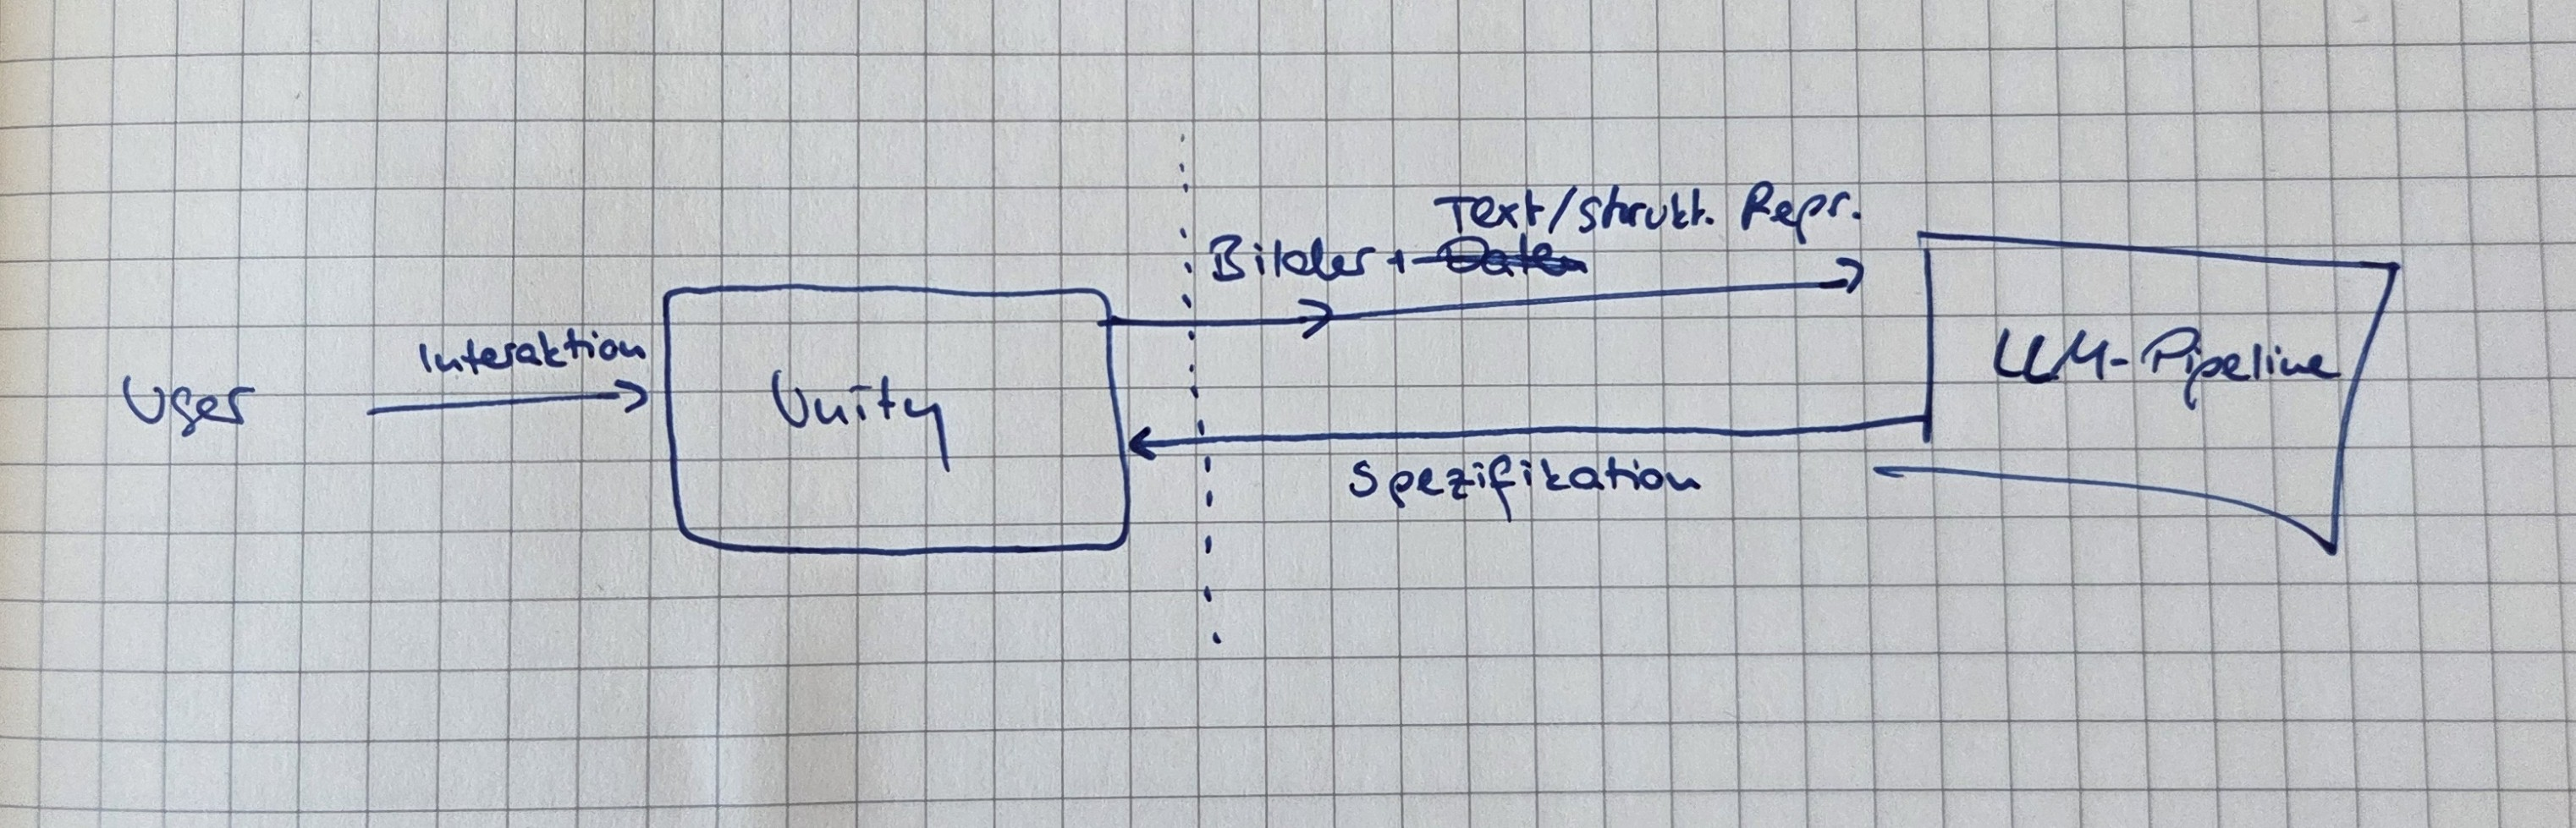
\includegraphics[width=0.8\linewidth]{figures/20260430_115502}
    \caption{Systemkontextdiagramm des VSG.}\label{fig:systemkontextdiagramm_vsg}
\end{figure}

Unity-Prozesse übersetzen das ausgewählte 3D-Objekt zudem in Formate, die von nachgelagerten Modulen und insbesondere den darin enthaltenen LLMs entgegengenommen werden können und zeigt die geplanten Interaktionen an, damit diese von Benutzer*innen bestätigt oder in einer Iterationsschleife korrigiert werden können. Dieser Human-in-the-Loop-Schritt adressiert A5.
Zusätzlich ist Unity die Umgebung, in der Vivian die Anreicherung eines statischen 3D-Assets mit Interaktionslogik über Spezifikationsdateien zur Laufzeit leistet.
Nach erfolgreicher Generierung der Vivian-Spezifikation liefert die KI-Pipeline diese zurück an Unity, damit dort Vivian zusammen mit statischem 3D-Asset und dieser Spezifikation ausgeführt werden kann.
Diese Gesamtarchitektur adressiert A1, da aus natürlichsprachlichen Eingaben und bestehenden Szenenrepräsentationen vollständige Vivian-Spezifikationen erzeugt werden.

Weiterhin erfolgt die Kommunikation der KI-Pipeline mit Unity über eine REST-API-Schnittstelle, sodass Funktionalitäten der Pipeline gegebenenfalls durch weitere Endpunkte erweiterbar bleiben.
Durch diese Entkopplung könnte die KI-Pipeline auch in einen übergeordneten Prozess integriert werden, ohne an die Unity-UI gebunden zu sein.

\section{Verwendete Sprachmodelle und Agenten}

%Technisch kannst du erwähnen, dass output_type=SceneUnderstanding die Ausgabe in eine Pydantic-Struktur zwingt. Die OpenAI-Agents-Dokumentation beschreibt, dass ein Agent über output_type statt Freitext einen bestimmten Ausgabetyp, z. B. ein Pydantic-Objekt, erzeugen kann und dabei Structured Outputs verwendet werden . Die Structured-Outputs-Dokumentation beschreibt außerdem, dass Antworten an ein vorgegebenes JSON-Schema gebunden werden können .

\section{Gesamtpipeline und Datenfluss}


\begin{figure}[htbp]
    \centering
    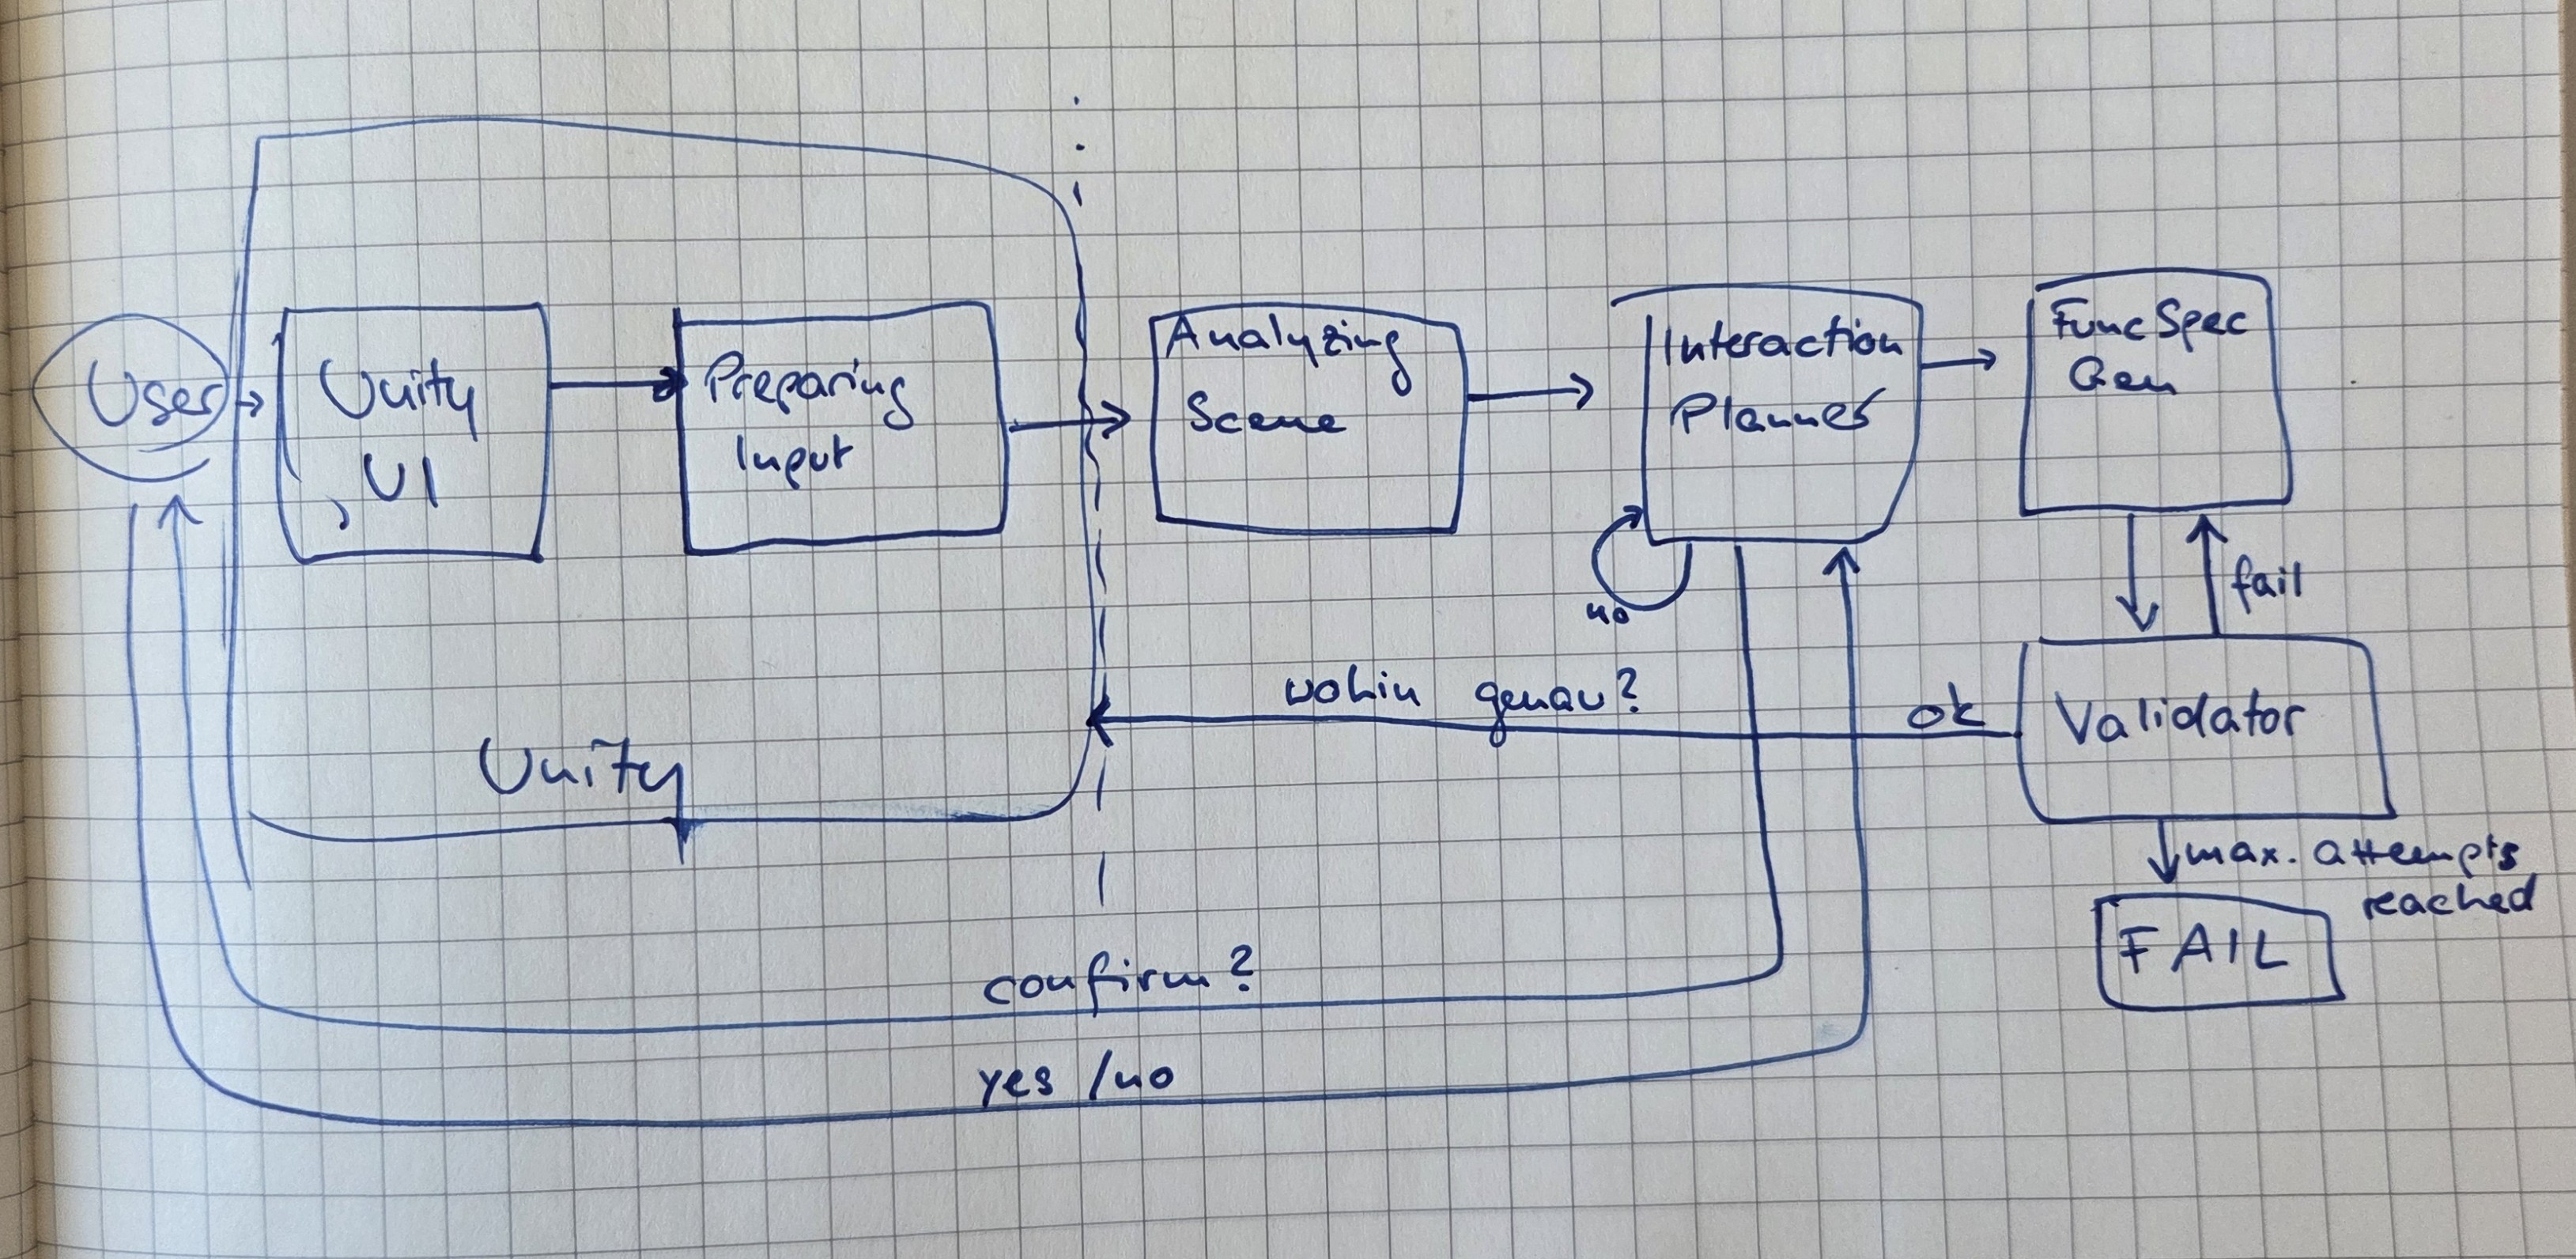
\includegraphics[width=0.8\linewidth]{figures/20260430_120448}
    \caption{Container-Diagramm des VSG.}\label{fig:containerdiagramm_vsg}
\end{figure}

Ein*e Benutzer*in kann über die Unity UI mit dem System interagieren und erhält Informationen über den Prozessfortschritt, Logging-Informationen, Rückmeldung des Interaktionsplaners und ob ein Durchlauf erfolgreich war.
Anschließend wird das ausgewählte 3D-Asset über ein weiteres Unity-Skript in eine strukturelle Szenenrepräsentation umgewandelt sowie ergänzende 2D-Bildansichten gerendert.

Diese aufbereitete Szenendarstellung wird im darauffolgenden Schritt zusammen mit einer initialen Benutzer*innenbeschreibung der gewünschten Interaktivität an den Scene Analyzer übermittelt.
Dieser gibt ein Scene-Understanding-Objekt aus, welches für jedes relevante Objekt dessen Funktion, Rolle und Eignung als potenzielles Interaktions- oder Visualisierungselement enthält.

Anschließend erhält der Interaction Planner das zuvor generierte Scene-Understanding-Objekt zusammen mit der strukturierten Szenenrepräsentation, die zuvor auch der Scene Analyzer erhalten hat, und der natürlichsprachlichen Interaktionsbeschreibung.
In diesem Schritt wird geplant, welche Interaktions- und Visualisierungselemente es geben wird, welche Zustände der Prototyp einnehmen kann und welche Übergänge zwischen Zuständen vorgesehen sind.
Der Interaction Planner gibt einen Interaction-Plan aus, welcher Element-Rollen, geplante Zustände und Übergänge sowie eine Liste der zu generierenden Spezifikationsdateien enthält.
Dieser Plan wird gemäß A5 der Benutzer*in anschließend zur Bestätigung oder Korrektur vorgelegt.
Bei einer Korrektur wird der Interaction Planner erneut aufgerufen, um diese anzuwenden, bis der Plan bestätigt wird, welcher schließlich den nachgelagerten Modulen als verbindliche Vorgabe dient.

Der Specification Generator erzeugt auf Grundlage dieses Interaktionsplans die eigentlichen Vivian-Spezifikationsdateien in der notwendigen Reihenfolge.
Ausgegeben werden vier strukturierte JSON-Dateien, welche zusammen eine Vivian-Spezifikation bilden.

Der Consistency Reviewer prüft nun mithilfe des Interaktionsplans, ob der Plan korrekt vom Specification Generator umgesetzt wurde und ob logische Widersprüche oder dateiübergreifende Inkonsistenzen existieren.
Das könnten \zB~unerreichbare Zustände oder widersprüchliche Bedingungen sein, welche eine rein strukturelle Validierung nicht erkennen kann

Ein Validator ergänzt dies um eine strukturelle und laufzeitnahe Kontrolle.
Wird die maximale Anzahl an Versuchen erreicht oder keine Fehler gefunden, terminiert der VSG.
Letzteres sorgt für ein Zurückliefern der generierten Vivian-Spezifikation an Unity, sodass Vivian diese zusammen mit dem statischen 3D-Asset ausführen kann.

% Als nächstes:
% -	Abgrenzung zu anderen systemen
% -	In-detail: was macht jedes modul und v.a. WIE funktioniert es?
% -	Fixer Agent nochmal genau überprüfen und ggf. in extra absatz, wenn der tatsächlich ne tragende rolle spielt? Und wird fixer agent auch ausgeführt, wenn Consisttency reviewer fehler erkennt?
% - unity ui einbinden

% Dann schreib einen einzigen Absatz (ca. 150–200 Wörter) zu einem Modul deiner Wahl – das, das du am besten verstanden hast. Stichpunktartig genügt: Eingabe, Ausgabe, welches Modell/welche Strategie, welche Anforderung das adressiert. Du formulierst's danach aus.


%A3/A4 Validierung + self-correction funktionieren ohne klare grenzen zwischen modulen nicht sinnvoll
%Nicht erklären WIE jedes modul intern funktioniert, das gehört in modulabschnitte

% Ein Absatz Datenfluss von Eingabe bis Ausgabe: was geht rein (Szenenrepräsentation + natürlichsprachliche Beschreibung), was passiert in welcher Reihenfolge, was kommt raus (Vivian-Spec). Hier nennst du die Module beim Namen und sagst in einem Satz, was jedes tut – aber noch keine Details, das kommt in den späteren Modulabschnitten. Lieber drei Sätze pro Modul als zehn.

% Zwischenartefakte und Kontrollfluss: welche Daten zwischen den Modulen wandern (Szenenanalyse-Ergebnis, Interaktionsplan, Spezifikationsentwurf, Validierungsbericht), wo die Validierungs-Gates sitzen (vor und nach Generierung), und wo der HITL-Schritt eingreift (vor Spec-Generierung, gemäß A5). Das ist der Absatz, der dein Diagramm in Worte übersetzt.

% Ein Absatz Abgrenzung: kurzer Vergleich zu LLMR / HOLODECK / ArtiWorld – jeweils zwei Sätze, was übernommen wird (z. B. modulare Inspection von LLMR), was bewusst anders ist (du erzeugst keine Geometrie, du fügst Verhaltens-Spezifikationen zu vorhandenen Szenen hinzu). Damit verteidigst du implizit deinen Beitrag.

% REST API -> WIE kommuniziert unity mit ki-pipeline? 


% welches sprachmodell für welches modul? klein bis groß

\section{Vorverarbeitung in Unity}\label{sec:vorverarbeitung_unity}


%TODO warum überhaupt vorverarbeiten?
Um ein 3D-Asset in MLLM-verständliche Daten umzuwandeln, müssen eine strukturelle Repräsentation und Ansichten aus verschiedenen Blickwinkeln erstellt werden.
Da der nachgelagerte Scene Analyzer mit Text und Bild als Eingaben arbeitet, benötigt er die erstellten Ansichten als visuelles Grounding für die abstrakten JSON-Daten.
Die Form des Objekts, das Material oder auch räumliche Anordnung werden somit direkt sichtbar und müssen nicht aus Bounding-Boxen rekonstruiert werden.

Im ersten Schritt wird dazu aus dem im Unity-Fenster (Abbildung~\ref{fig:unity_ui_empty}) ausgewählten 3D-Asset ein \textit{Prefab}-Objekt erzeugt, welches später von Vivian zur Laufzeit instanziiert wird.
Damit wird gemäß D2 keine neue Geometrie generiert, sondern wiederverwendet.

\begin{figure}[htbp]
    \centering
    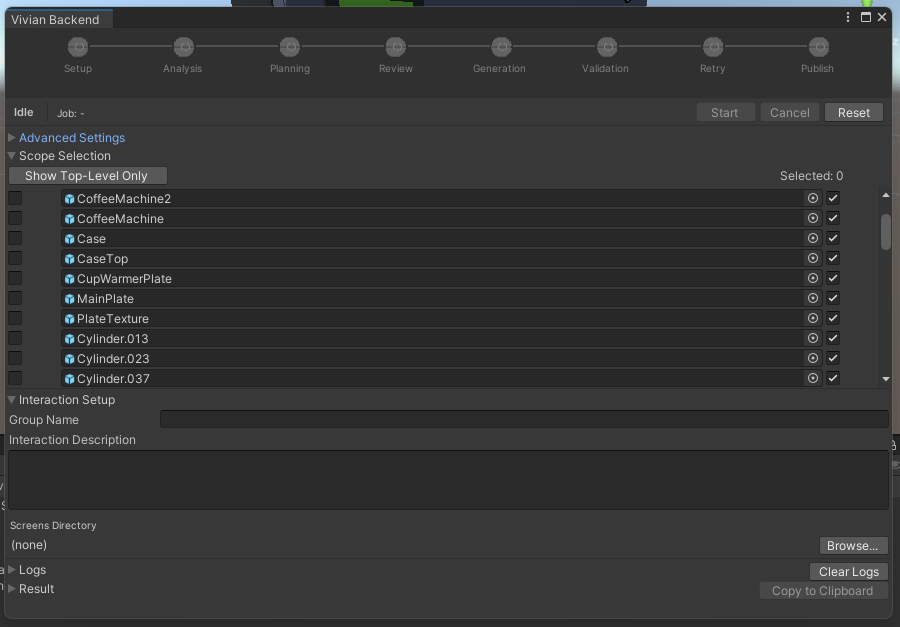
\includegraphics[width=0.8\linewidth]{figures/unity-ui}
    \caption{Unity UI des VSG.}\label{fig:unity_ui_empty}
\end{figure}

Um einem LLM Verständnis über ein 3D-Asset (in Unity\glqq GameObject\grqq{} genannt) zu geben wird zunächst eine strukturierte Szenenbeschreibung im JSON-Format mit dem Namen \textit{scene.json} erzeugt.
Dazu wird die Hierarchie des Szenengraphen rekursiv traversiert und pro GameObject Informationen wie die ID, der Hierarchiepfad, Transformation, Materialien, Bounding Boxes oder Mesh-Statistiken extrahiert.
Weiterhin werden bereits basierend auf Namen, Tags oder Material-Hinweisen heuristisch Rollen erkannt, welche im späteren Verlauf verwendet werden können, um Interaktionselemente und Visualisierungselemente zu klassifizieren.

Im Anschluss daran rendert Unity für das übergeordnete GameObject verschiedene Ansichten, da die Erkennungsleistung eines MLLM steigt, wenn statt einer Einzelansicht mehrere gerenderte Ansichten eines 3D-Objekts verwendet werden~\cite{suMultiviewConvolutionalNeural2015}.
Dafür werden sechs orthografische Ansichten entlang der Hauptachsen sowie zwei isometrische (von schräg oben) als 1024x1024-Pixel-PNGs erstellt (siehe Abbildung~\ref{fig:toaster_views}).
Die gewählte Anzahl der Ansichten ist ein Kompromiss zwischen Erkennungsrobustheit und minimal notwendigem Bildumfang, um Kosten pro Durchlauf zu sparen.
Die orthografischen Ansichten vermeiden perspektivische Verzerrung und beinhalten saubere Silhouetten, während die isometrischen Ansichten die räumliche Gesamtform und Lesbarkeit verbessern sowie drei Raumdimensionen in einer Darstellung erfassbar machen.
Zur Laufzeit wird dazu eine Kamera angelegt, anhand der Welt-Bounding-Box des Objekts platziert und auf das Objektzentrum ausgerichtet.
Alle dafür benötigten Ressourcen werden anschließend wieder freigegeben.

\begin{figure}[htbp]
    \centering
    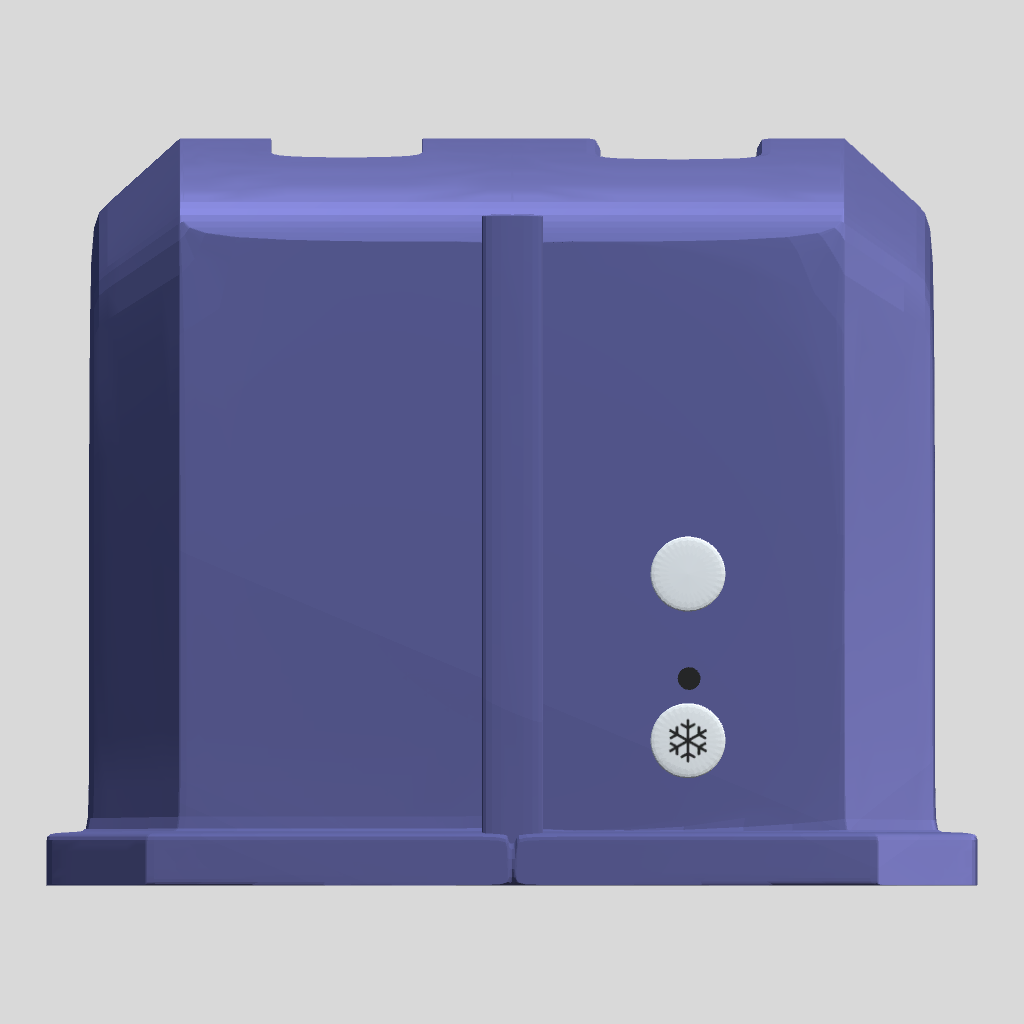
\includegraphics[width=0.22\linewidth]{figures/toaster_views/toaster3_front}\hfill
    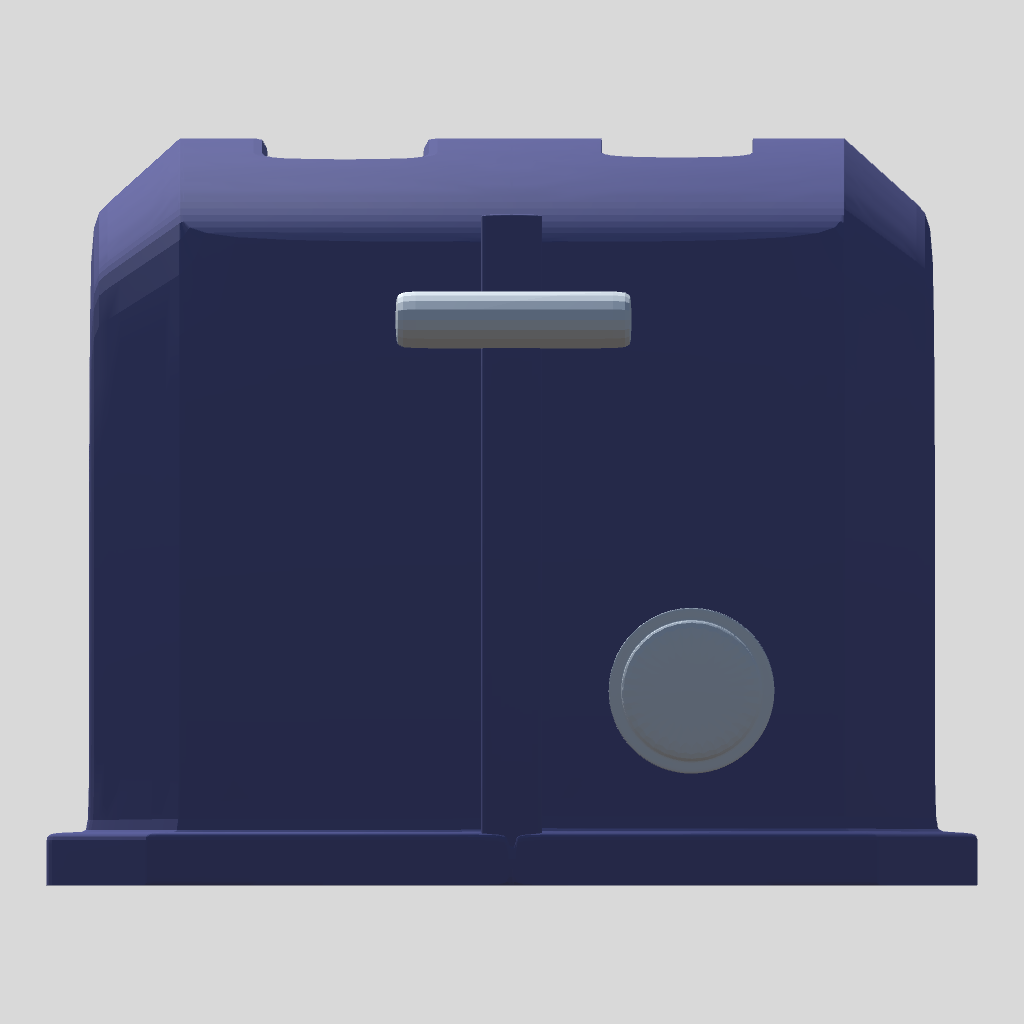
\includegraphics[width=0.22\linewidth]{figures/toaster_views/toaster3_back}\hfill
    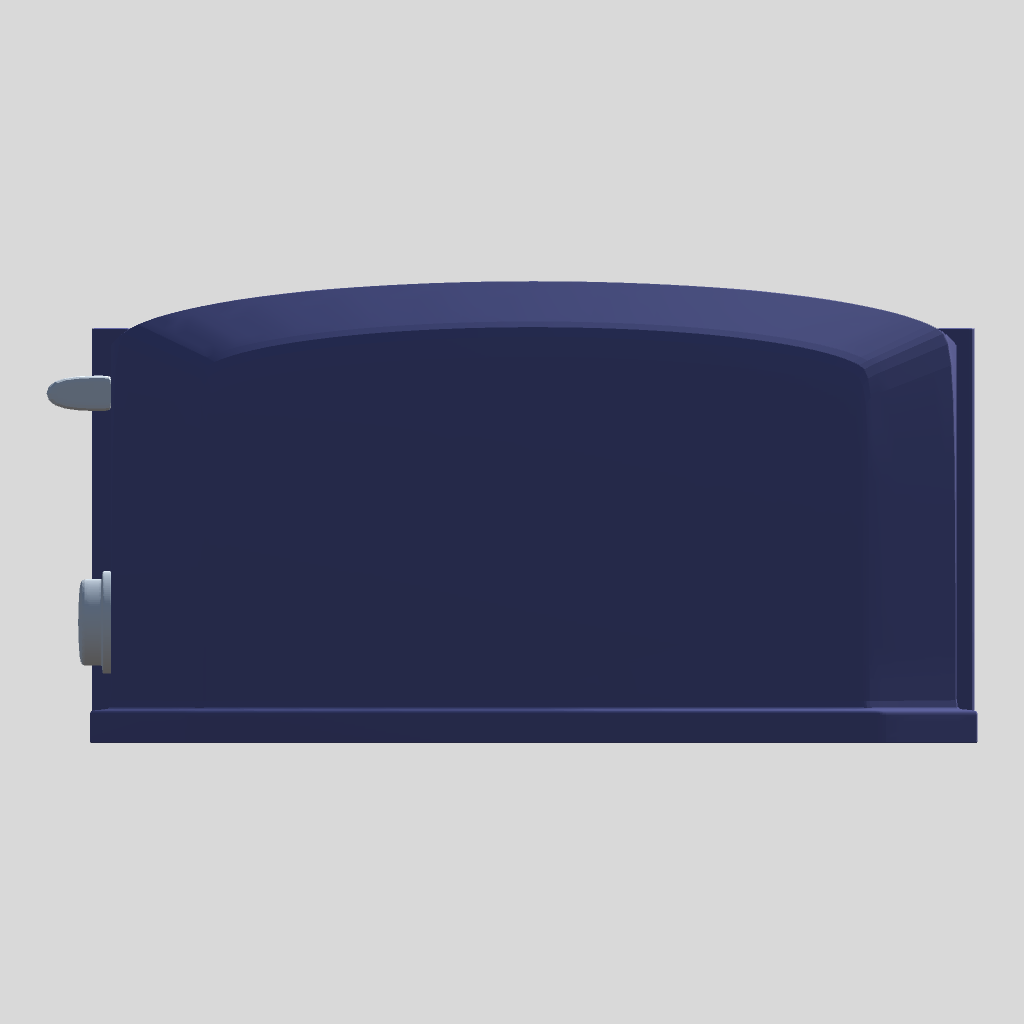
\includegraphics[width=0.22\linewidth]{figures/toaster_views/toaster3_left}\hfill
    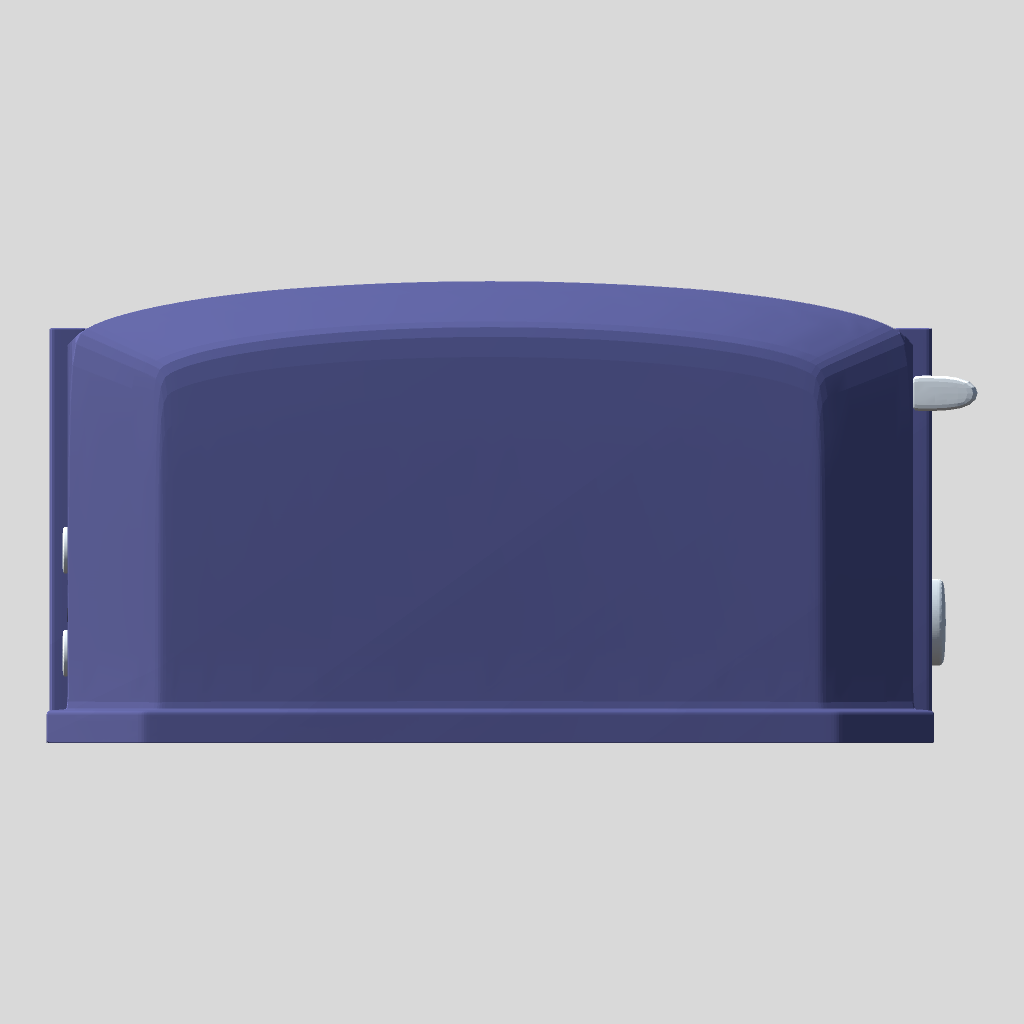
\includegraphics[width=0.22\linewidth]{figures/toaster_views/toaster3_right}\\[1em]
    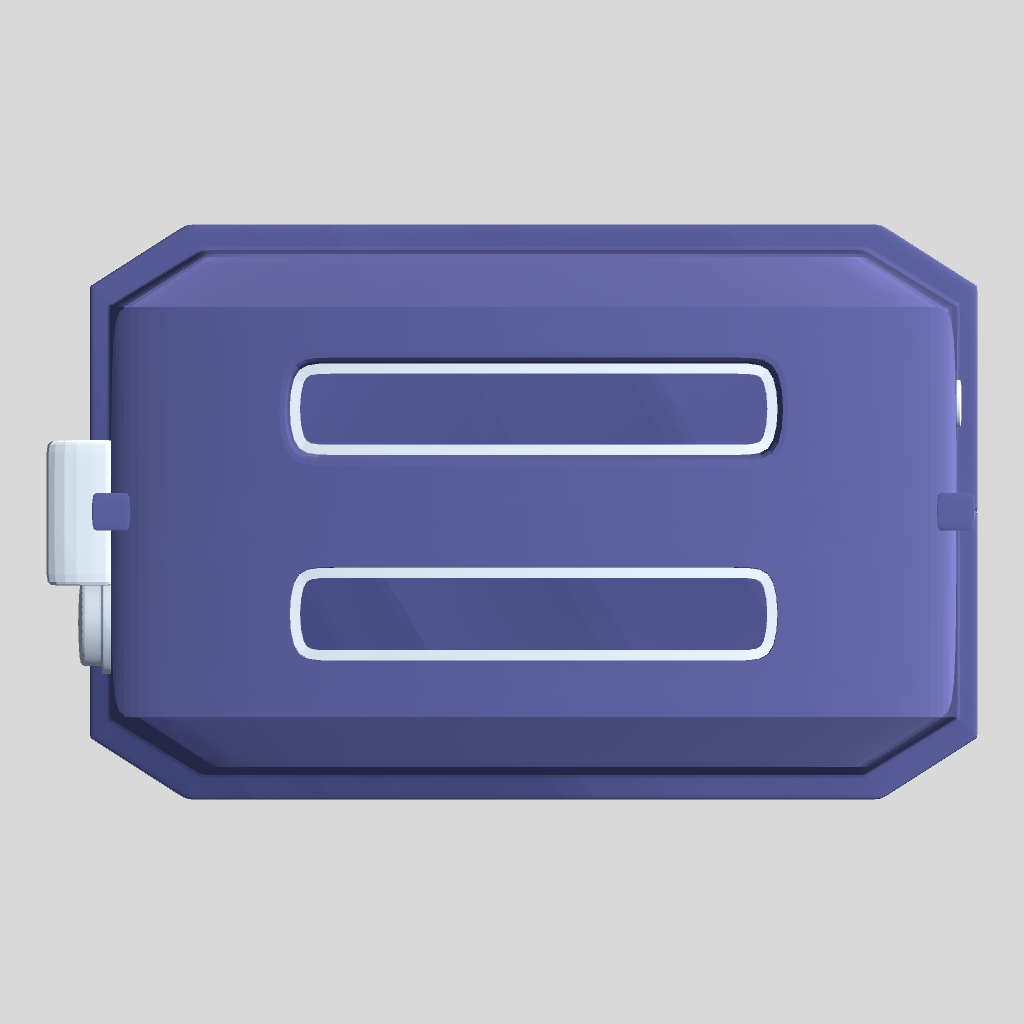
\includegraphics[width=0.22\linewidth]{figures/toaster_views/toaster3_top}\hfill
    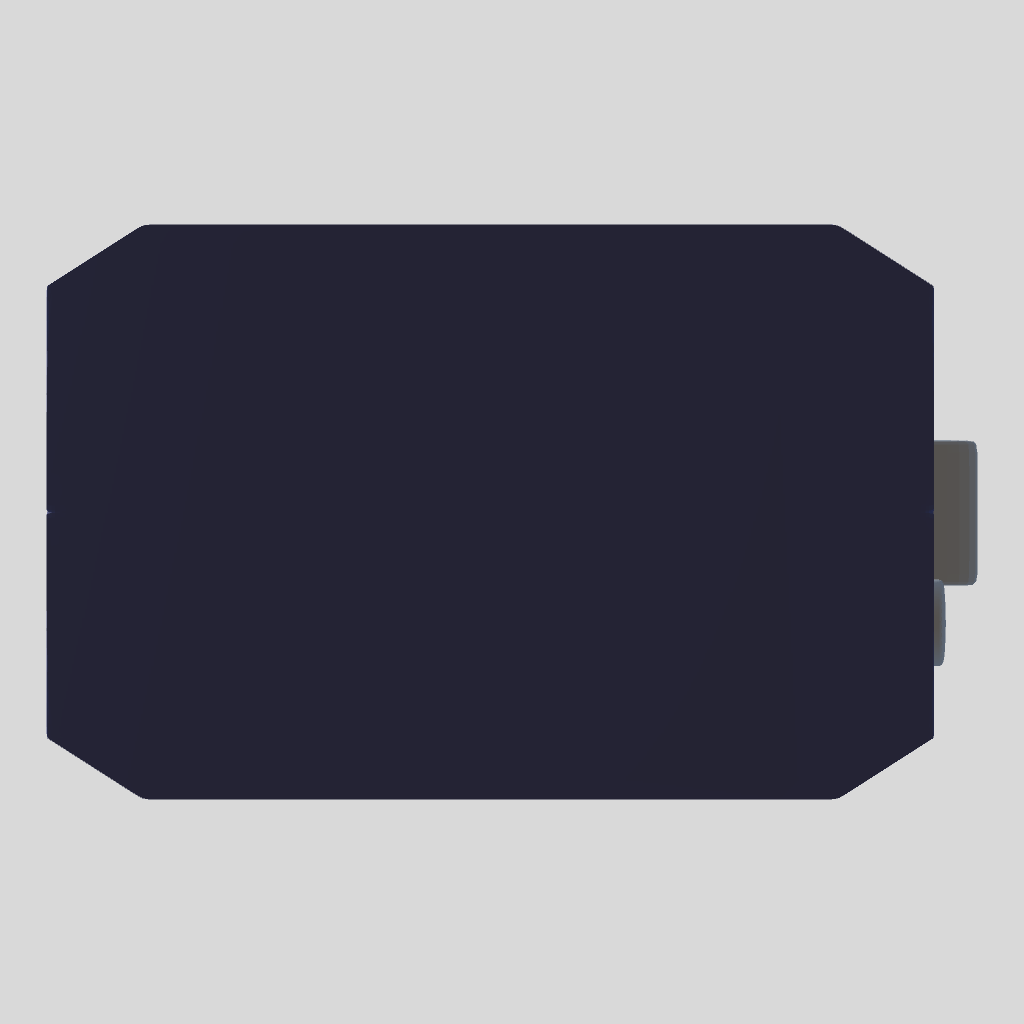
\includegraphics[width=0.22\linewidth]{figures/toaster_views/toaster3_bottom}\hfill
    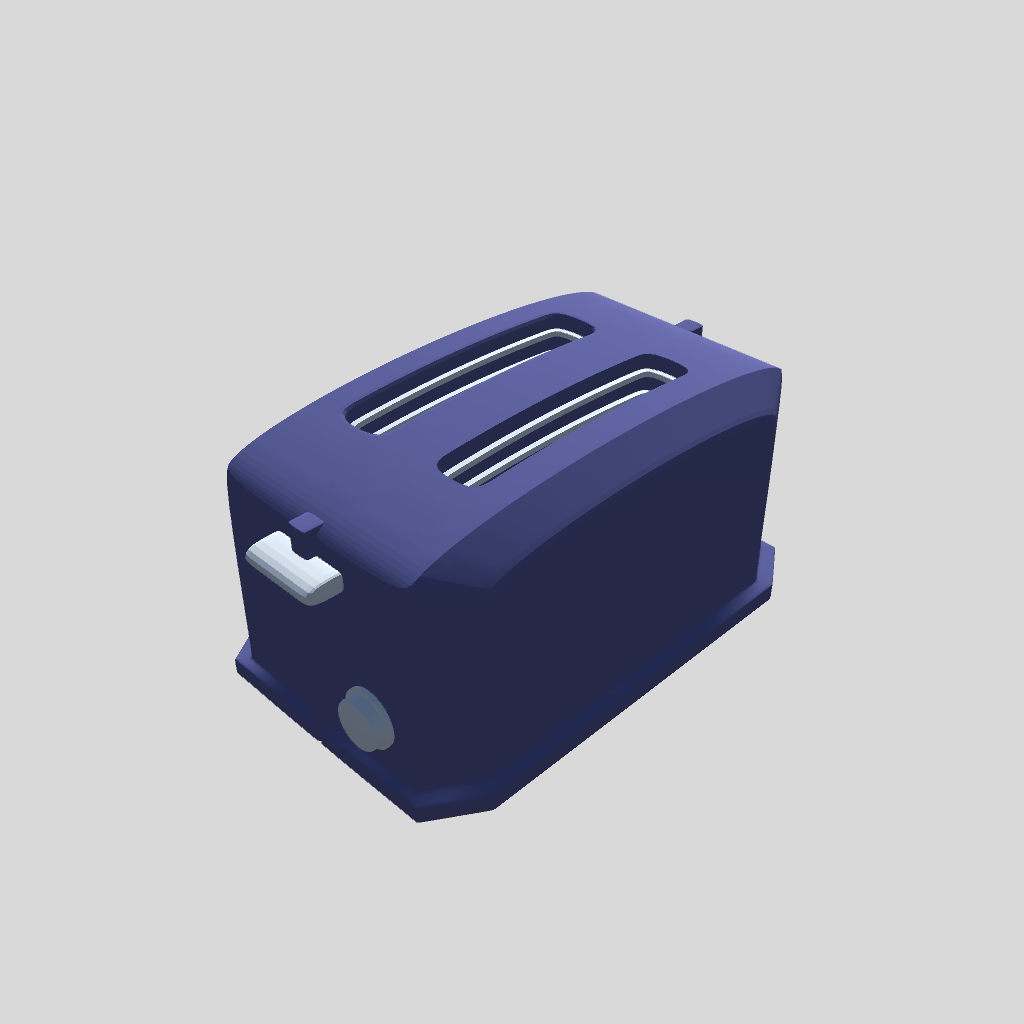
\includegraphics[width=0.22\linewidth]{figures/toaster_views/toaster3_iso_top_left}\hfill
    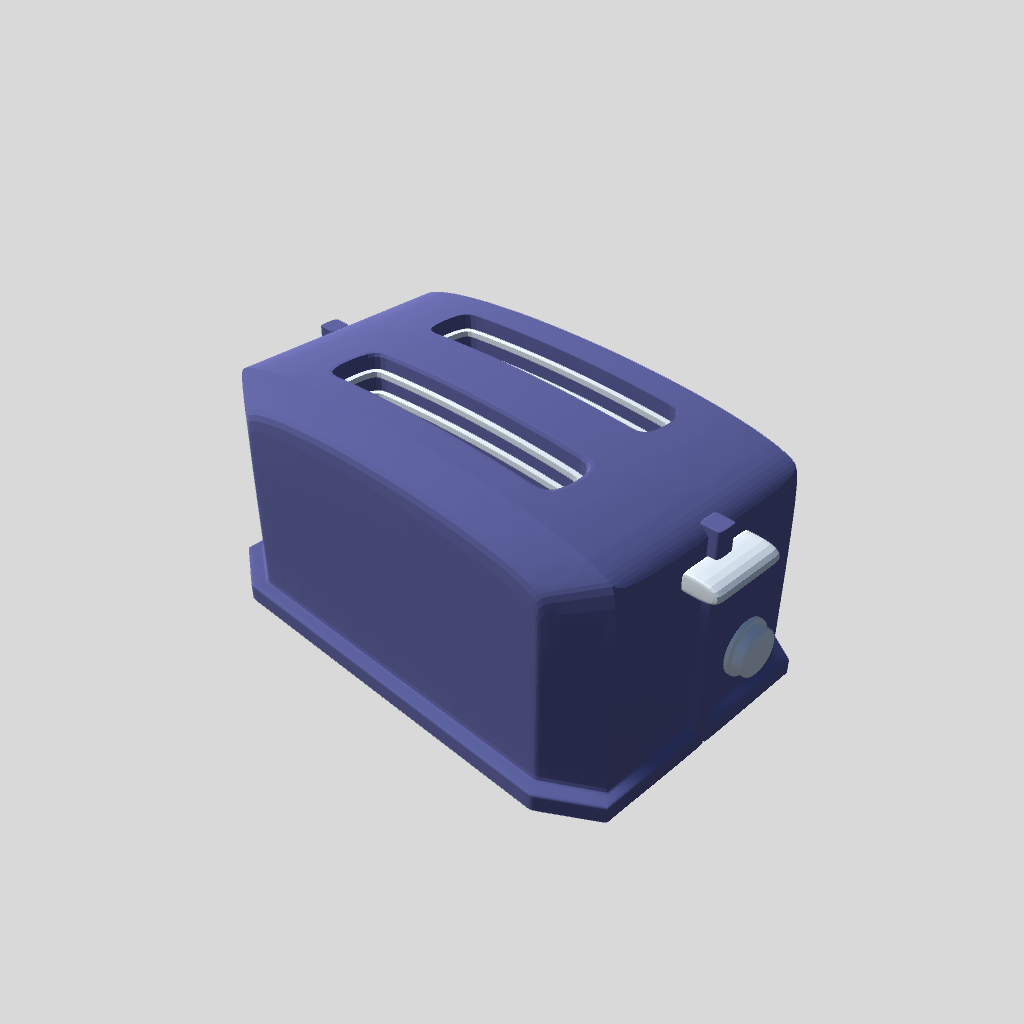
\includegraphics[width=0.22\linewidth]{figures/toaster_views/toaster3_iso_top_right}
    \caption{Acht gerenderte Ansichten eines Toaster-3D-Assets.}\label{fig:toaster_views}
\end{figure}

Eine zugehörige Datei namens \textit{views\_manifest.json} enthält pro Bild Kameramatrizen, Pose, Projektionstyp und einen Vermerk, welches Teilobjekt des Szenengraphen sich an welcher Stelle in der Ansicht befindet.
Unity kennt die Kameraposition die 3D-Box jedes Objekts in der Szene und kann so ausrechnen, wo sich ein Objekt der Szene im jeweiligen Bild befindet.
Nachgelagerte MLLMs können so den Zusammenhang zwischen Objekten in \textit{scene.json} und denen aus den Ansichten (siehe Abbildung~\ref{fig:toaster_views}) herstellen.
Dafür wird die ID, ein Tiefenhinweis und das Pixelrechteck vermerkt, in dem sich das Objekt im Bild befindet.

Der Vorverarbeitungsschritt in Unity erzeugt also zusammengefasst aus einem vorhandenen, statischen 3D-Asset eine strukturelle Repräsentation als JSON-Struktur, acht gerenderte Ansichten von diesem sowie eine weitere JSON-Struktur mit Informationen zu den Ansichten.
Diese Daten können nun vom nächsten Modul, dem Scene Analyzer, konsumiert werden.
In diesem Schritt werden D2, D4 sowie N1 adressiert, da Geometrie erhalten bleibt, die JSON-Struktur eine Basis für spätere Namensreferenzen bietet und definierte Ein- und Ausgabeformate verwendet werden.

% \subsection{Modul Beispiel}
% Das Modul zur Interaktionsableitung übersetzt die semantische Beschreibung eines statischen 3D-Assets in eine strukturierte Beschreibung möglicher Interaktionen. Es adressiert insbesondere die Anforderungen A2, A4 und A6. A2 fordert die Identifikation potenziell interaktiver Teilobjekte, A4 die Ableitung geeigneter Zustände und Transitionen und A6 die Ausgabe in einem maschinenlesbaren Format.

% Konzeptionell wurde das Modul als Zwischenschritt zwischen Szenenanalyse und Spezifikationsgenerierung entworfen. Dadurch wird vermieden, dass die finale Vivian-Spezifikation direkt aus unstrukturierten Eingabedaten erzeugt wird. Stattdessen entsteht zunächst eine abstrakte Interaktionsbeschreibung, die unabhängig vom konkreten Ausgabeformat geprüft und weiterverarbeitet werden kann.

% Implementiert wurde das Modul durch eine LLM-gestützte Analyse der Objektstruktur. Als Eingabe erhält es die extrahierte Hierarchie des Unity-Modells, begleitende Objektinformationen sowie die natürlichsprachliche Nutzerbeschreibung. Die Ausgabe besteht aus einer strukturierten Liste potenzieller Interaktionselemente, Zustände und Übergänge, die anschließend vom Spezifikationsgenerator in die benötigten JSON-Dateien überführt wird.

% Module:
% | Bestandteil                 | Inhalt                                                  |
% | --------------------------- | ------------------------------------------------------- |
% | Zweck des Moduls            | Welche Aufgabe übernimmt das Modul in der Pipeline?     |
% | Zugeordnete Anforderungen   | Welche Anforderungen werden durch das Modul adressiert? |
% | Konzeptionelle Entscheidung | Warum wurde das Modul so entworfen?                     |
% | Implementierung             | Wie wurde es technisch umgesetzt?                       |
% | Eingabe / Ausgabe           | Welche Daten erhält und erzeugt das Modul?              |
% | Grenzen                     | Was leistet das Modul bewusst nicht?                    |

\section{Scene Analyzer}

%noch genauer auf LLM prompt eingehen

Die Kernaufgabe des Scene-Analyzer-Moduls besteht darin, die in der Vorverarbeitung entstandenen visuellen Eindrücke und strukturellen Daten mit der natürlichsprachlichen Nutzer*innenbeschreibung zu verknüpfen und die rohen Daten so in ein semantisch angereichertes Zwischenformat zu überführen. F2 wird hier adressiert, da relevante Objekte und Teilobjekte aus Szeneninformationen und der Beschreibung abgeleitet werden, sodass nachfolgende Schritte auf diese referenzieren können.

Als Eingaben bekommt der Scene Analyzer die in Abschnitt~\ref{sec:vorverarbeitung_unity} beschriebene strukturierte Szenenrepräsentation und die Ansichten des Objekts.
Die JSON-Struktur stellt Namen, Pfade, IDs und Geometrie bereit, während die Bilder bei der semantischen Einordnung helfen.
Diese Daten werden von einem internen LLM-basierten Agenten verarbeitet, welcher so einordnen kann, ob ein Teilobjekt beispielsweise eher Griff, Display oder Knopf ist.

Das verwendete LLM leistet in diesem Modul die Hauptarbeit: Es klassifiziert die Szeneninformationen gemäß einem vorgegebenen Schema, dem \textit{SceneUnderstanding}.
In Anhang~\ref{sec:anhang_scene_analysis_instructions} ist dargestellt, wie der verwendete Agent mithilfe eines strukturierten Prompts angesteuert wird.
%TODO anhang prompt hinzufügenssd
Bei Verwendung von OpenAI-Agenten besteht die Möglichkeit, einen bestimmten Ausgabetypen (\textit{output\_type}) festzulegen anstelle von Freitext.
In diesem Fall wird ein \glqq Pydantic\grqq{}-Modell als \textit{output\_type} festgelegt, sodass das LLM in genau diesem Schema antwortet.

Dieses \textit{SceneUnderstanding} beinhaltet nun ein aufbereitetes Szenenverständnis mit Informationen zu Objektbezügen, Relationen oder Clustern und bietet die Grundlage dafür, dass darauffolgende Agenten ein Verhalten aus der analysierten Szene ableiten können. Durch dieses Zwischenprodukt muss der Interaction Planner nicht direkt aus einer Unity-Hierarchie schließen, welche Objekte funktional relevant sind, sondern kann mit einer semantisch vorstrukturierten Repräsentation arbeiten.

Diese entstandene kontrollierte Zwischenrepräsentation ist maschinenlesbar und validierbar, bleibt allerdings dennoch von der Qualität der Modellinterpretation abhängig und ist anfällig für semantische Falschannahmen, weshalb spätere Review-Schritte relevant bleiben.


\section{Interaction Planner}
Dabei ist auch zu berücksichtigen, welche Spezifikationsdateien überhaupt benötigt werden, da sehr simple Prototypen, wenn überhaupt, weniger Zustände als komplexere Prototypen benötigen.
Für das in diesem Modul eingebundene LLM ist also fundamentales Wissen über das Vivian-Framework von zentraler Bedeutung, da alle weiteren Module nach diesem Plan arbeiten.
(AUSFORMULIEREN/NEU PLATZIEREN: Durchläufe ohne dieses Modul haben gezeigt, dass unnötige Zustände/Übergange generiert wurden, die nicht nötig gewesen wären, z.B. weil das Asset sehr simpel war. Beleg?).

\section{Specification Generator}
Er ist in vier nacheinander ausgeführte, jeweils auf einen Teil der Spezifikation spezialisierte LLM-Agenten zerlegt: Interaktionselemente, Visualisierungselemente, Zustände und Übergänge. Diese Reihenfolge entspricht den Abhängigkeiten zwischen den Dateien: Jeder Agent erhält neben dem bestätigten Interaktionsplan und der Szenenrepräsentation auch die Ausgaben der vorangegangenen Agenten als Kontext und referenziert deren konkrete Element- sowie Zustandsnamen.
Nach der Generierung jeder Teilspezifikation wird diese bereits auf referenzielle Fehler kontrolliert (siehe A3). Auch diese Agenten benötigen fundiertes Wissen über das Vivian Framework und klare Regeln, nach denen sie Entscheidungen treffen. Dieser Schritt adressiert die Anforderungen A1, D1, D3 sowie D4 und bietet die Grundlage für A4, da einzelne Teilschritte des Specification-Generators durch diesen Aufbau gezielt erneut ausgeführt werden können.

In diesem Schritt wird ebenfalls eine VisualizationArrays.json-Datei ohne Inhalt erzeugt, welche zur Ausführung von Vivian benötigt wird, aber für die in diesem System betrachtete Prototypenerstellung keine weitere Relevanz hat und daher im Folgenden unerwähnt bleibt.
Eine Vivian-Spezifikation gilt somit in dieser Arbeit als vollständig, wenn sie InteractionElements.json, VisualizationElements.json, States.json und Transitions.json enthält.

\section{Consistency Reviewer}
Ein Consistency-Reviewer erhält die Spezifikationsdateien sowie den Interaktionsplan, da hier mit Hilfe eines weiteren LLM-Agenten geprüft wird, ob die geplanten Interaktionen tatsächlich umgesetzt sind.

Ein Unity-Validator ergänzt dies um eine strukturelle und laufzeitnahe Kontrolle, wodurch tatsächliche Initialisierungsfehler bereits vor der Übermittlung an Unity aufgedeckt werden können. Dieser Schritt adressiert A3.

\section{Validator}

Sollten Fehler im Unity-Validator aufkommen, gibt dieser eine strukturierte Fehlerliste an einen Reparatur-Agenten (Fixer Agent) weiter, welcher über einen Reparaturplan eine gezielte Wiederausführung der betroffenen Agenten im Specification-Generator einleitet. So kann eine vollständige Neugenerierung der Spezifikation vermieden werden. Dieser Teilschritt adressiert A4.